\documentclass[fr]{../../../eplsummary}

\hypertitle{Stratégie d'entreprise}{6}{ECGE}{1315}
{Guillaume Prieur}
{Alain Vas}

\renewcommand{\it}[1]{\textit{#1}}
\renewcommand{\bf}[1]{\textbf{#1}}
\newcommand\tab[1][1cm]{\hspace*{#1}}
\newcolumntype{x}[1]{>{\centering\let\newline\\\arraybackslash\hspace{0pt}}p{#1}}
\newtheorem*{ex}{Exemple}

\newpage
\section*{Note}
Le cours ayant beaucoup changé, cette synthèse est une nouvelle version de la synthèse de Florian Thuin. Vous pouvez trouver l'ancienne synthèse au commit 849b114 à l'adresse\\
\\
\url{https://github.com/Gp2mv3/Syntheses/tree/b0f20a0df8d62fd5c829e736d1826913c6ea48b0/src/q6/strat-ECGE1315/summary}\\
\\
Cette synthèse se base essentiellement sur l'excellent livre \it{Les fondements de la stratégie} de Alain Vas aux éditions DUNOD. Il reprend les schémas et les dessins du livre (à savoir les Figures \ref{chaine_de_valeur}, \ref{ansoff} et \ref{bcg}) pour illustrer certains passages de la synthèse. Toutes les autres images sont tirées des Powerpoints du cours LECGE1315 - Stratégie d'entreprise dispensé à l'Université Catholique de Louvain-La-Neuve par le Professeur Alain Vas.
\section{Introduction à la stratégie}
\subsection{Définition de la stratégie}
Dans un premier temps, nous pouvons définir le concept de stratégie comme les finalités et l’orientation à long terme d’une organisation. Elle porte sur les décisions délibérées et rationnelles que prend une entreprise pour créer de la valeur pour pour ses clients et l'ensemble de ses parties prenantes. Typiquement, une stratégie consiste à développer un avantage concurrentiel durable.
\subsection{Les logiques stratégiques "FIT" ou "STRETCH"}
Les réflexions stratégiques se sont polarisées autour de deux grandes écoles de pensées : la logique "FIT" et la logique "STRETCH." Ces deux stratégies se valent l'une comme l'autre. Néanmoins, il faut choisir une des deux stratégies et être conscient de son choix. Un changement de logique peut tout de même s'opérer au cours du temps.
\subsubsection{La logique "FIT"}
Si l'entreprise adopte la logique "FIT", sa réflexion stratégique débute par l'analyse de l'environnement externe. L'organisation définit les moyens dont elle a besoin pour atteindre les objectifs visés.
\begin{ex}[Oréal]
L'Oréal repère les nouvelles opportunités sur les différentes continents et va développer des produits spécifiques qui répondent aux attentes des nouveaux consommateurs
\end{ex}
Cette logique se résume en 5 étapes.
\begin{enumerate}
    \item Identification des marchés potentiels,
    \item identification des sources de profits possibles,
    \item évaluation de la concurrence,
    \item évaluation d'une stratégie opérationnelle,
    \item et détermination des efforts à fournir.
\end{enumerate}
Cette logique permet de capter une rente dite de monopole. Elle repose sur un rationnement du marché.
\subsubsection{La logique "STRETCH"}
Dans la logique "STRETCH", l'entreprise part cette fois de l'analyse du potentiel de création de valeur que ses propres ressources et compétences peuvent procurer et les traduit en en marchés. 
\begin{ex}[Dyson]
L'entreprise a créé l'aspirateur à sac en ayant une réflexion sur les technologie et les usages. Elle a décidé de proposer autre chose aux consommateurs.
\end{ex}
Cette logique se résume également en 5 étapes.
\begin{enumerate}
    \item Identification des potentialités de création,
    \item évaluation du potentiel-profit,
    \item estimation de la capacité des offres,
    \item élaboration d'une stratégie,
    \item et identification des efforts à fournir.
\end{enumerate}
Cette logique permet de capter une rente dite ricardienne. Elle repose sur la rareté de l'offre.
\subsection{Mission, vision et valeurs}
\subsubsection{La mission}
La mission est en quelque sorte l'ADN de l'entreprise. Elle définit que l'organisation fait et comment elle le fait. Elle permet de la guider dans les choix stratégiques en étant garant d'une cohérence d'ensemble. Elle facilite donc les prises de décision.
\begin{ex}[Google]
"Organiser à l'échelle mondiale les informations dans le but de les rendre accessibles à tous."
\end{ex}
Aujourd'hui, il existe une tendance à remplacer l'exercice de la mission stratégique par l'élaboration d'un Mantra. Ce dernier est plus court\footnote{Généralement, il ne dépasse pas les 5 mots.} et simple. Il est facile à retenir. Il ne faut pas le confondre avec le slogan.
\begin{ex}[Nike]
La performance sportive authentique. A ne pas confondre avec le slogan "Just do it."
\end{ex}
L'idéal est de coupler un mantra et une mission.
\subsubsection{La vision}
La vision consiste à fixer des ambitions démesurées pour le futur par rapport à l'état actuel de l'entreprise et à ses ressources. Elle suppose donc de s'émanciper de ses conditions environnementales actuelles.
\begin{ex}[WWF]
"Arrêter la dégradation de l'environnement dans le monde et construire un avenir où les humains pourront vivre en harmonie avec la nature."
\end{ex}
La vision est un outil d'inspiration, culturel et de communication interne comme externe. Elle permet de mettre en place une priorisation des choix.
\subsubsection{Les valeurs}
Les valeurs sont des principes fondamentaux immuables dans le temps qui donnent du sens au fonctionnement de l'entreprise. Elles guident les normes et les comportements des membres qui composent l'organisation. Il existe plusieurs systèmes de valeurs qui peuvent coexister au sein d'une entreprise.
\begin{ex}[Oréal]
On retrouve des valeurs liées à  l'efficacité organisationnelle, la qualité relationnelle et l'identité de l'entreprise.
\end{ex}
Edgar Schein subdivise la culture organisationnelle, c'est-à-dire les valeurs partagées au sein de l'entreprise, en trois couches : 
\begin{enumerate}
    \item les artefacts qui sont divisés en trois catégories : physiques, comportementaux, verbaux ;
    \item les valeurs qui définissent ce qui a de l'importance et les normes de comportements qui clarifient ce qui est considéré comme normal ou anormal ;
    \item les croyances et hypothèses fondamentales sont des postulats qui vont de soi et sont donc inaccessibles consciemment.
\end{enumerate}
Il faut être vigilant lors de la mobilisation de certaines valeurs afin d'éviter deux risques majeurs : une décalage entre les valeurs annoncées et la réalité de fonctionnement de l'organisation, et la difficulté de mener des changements au sein de l'entreprise si on ne prend pas en compte ces dimensions culturelles souvent intangibles.
\subsection{Le diagnostic stratégique}
\subsubsection{La segmentation stratégique}
La segmentation stratégique se définit comme une technique d'analyse qui permet de regrouper différentes activités de l'entreprise en sous-ensembles homogènes appelés domaines d'activités stratégiques.\footnote{Par paresse, nous les appellerons DAS tout au long de la synthèse.}
\begin{ex}[Danone]
Le groupe Danone compte quatre DAS : les produits laitiers frais, les eaux en bouteille, la nutrition infantile, la nutrition médicale.
\end{ex}
La segmentation stratégique est un processus délicat. Elle fait d'ailleurs l'objet des deux chapitres suivants. Cependant, voyons d'abord une approche simple construite sur base de trois axes : clients, produits/services et la technologie.\footnote{Il faut bien garder en tête ces trois axes de manière simultanée. Sinon vous risquerez de ne pas saisir entièrement l'environnement dans lequel évolue une entreprise.} Il réside deux grandes difficultés dans la segmentation stratégique.\\
\\
La première est de trouver un nombre cohérent de DAS. Une segmentation trop fine, et la vision globale de l'organisation sera perdue. A contrario, une insuffisance de segmentation, et l'entreprise risque de réaliser des investissements mal adaptés et peu rentables.
\begin{ex}[Apple]
Quand Steve Jobs revient à la tête d'Apple, il simplifia la gamme de produits : "Pas plus de 4 produits !" disait-il.
\end{ex}
La seconde est le risque de s'enfermer dans une segmentation définie au préalable.\footnote{Trouver une bonne segmentation prend du temps. Le travail une fois fini, l'organisation risque d'essayer de s'y tenir le plus possible, à tort.} Sur la carte stratégique, il ne faut pas oublier la perméabilité et la temporalité des frontières. 
\begin{ex}[DEC]
Le PDG de DEC affirmait qu'il n'y avait aucune raison que les gens possèdent un ordinateur chez eux. Levez la tête et admirez comment il a fait long feu. L'entreprise à déposer son bilant quelques années plus tard.
\end{ex}
Un premier modèle proposé est le modèle SWOT (Strengths, Weaknesses, Opportunities et Threats) qui traite de l'analyse externe comme de l'analyse externe. Nous utiliserons ce modèle comme la colonne vertébrale du diagnostiques stratégique que nous enrichirons avec des modèles plus récents.
\section{L'analyse stratégique externe}
L'analyse externe porte sur l'environnement de l'entreprise. Celui-ci implique deux niveaux d'analyse : le macro-environnement et le micro-environnement.
\subsection{Le macro-environnement}
Les entreprises évoluent dans un environnement caractérisé comme VUCA (pour Volatility, Uncertainty, Complexity et Ambiguity). Il est donc nécessaire de connaître des techniques de prospective et de s'intéresser à l'évolution du macro-environnement. 
\subsubsection{L'analyse PESTEL}
L'une des méthodes d'audit repose sur le modèle d'analyse PESTEL. Il permet de sortir des réflexions à court terme pour se projeter dans le long terme. Ce modèle comporte six catégories.
\begin{enumerate}
    \item \bf{Les facteurs Politiques} portent sur les décisions prises par les gouvernements nationaux ou les instances internationales.
    \begin{ex}[Facteurs politiques]
    La stabilité gouvernementale, la politique fiscale, la régulation du commerce extérieur ou la protection fiscale.
    \end{ex}
    \item \bf{Les facteurs Économiques} concernent l'état de santé macro-économique des pays d'une zone géographique donnée.    
    \begin{ex}[Facteurs économiques]
    Les cycles économiques, l'évolution du PNB, le taux de croissance ou la politique monétaire.
    \end{ex}
    \item \bf{Les facteur Socio-culturels} se rapportent à l'évolution d'une population et de ses caractéristiques.
    \begin{ex}[Facteurs socio-culturels]
    L'évolution démographique, la pyramide des âges, la mobilité social ou les nouveaux modes de consommation.
    \end{ex}
    \item \bf{Les facteur Technologiques} englobent les avancées et les innovations technologiques au sens large. 
    \begin{ex}[Facteurs technologiques]
    Les investissements privés et publics dans la technologie, le taux de transfert, les nouvelles découvertes ou la vitesse de transfert.
    \end{ex}
    \item \bf{Les facteurs Environnementaux} concernent les préoccupations écologiques.
    \begin{ex}[Facteurs environnementaux]
    La réglementation et les contraintes écologiques, les nouvelles normes de protection de l'environnement ou la consommation d'énergie.
    \end{ex}
    \item \bf{Les facteurs Législatifs} traitent de l'évolution des cadres législatifs.
    \begin{ex}[Facteurs législatifs]
    Accès restreints à certains marchés, le droit du travail, le droit du commerce, la législation sur la santé, les normes de sécurité ou les monopoles.
    \end{ex}
\end{enumerate}
On peut donner deux variantes :  le modèle PEST où les facteurs écologiques et législatifs sont regroupés dans le facteur politique et le modèle STEEPLED où le facteur éthique et le facteur démographique sont pris en compte dans l'analyse.\\
\\
\subsubsection{La méthode des scénarios}
Le modèle PESTEL va permettre à l'entreprise de construire des scénarios plausibles d'évolution. Cette méthode des scénarios permet de repérer les opportunités et les menaces définies par le modèle SWOT, d'identifier des scénarios plausibles à l'évolution de l'entreprise et de soutenir la prise de décision dans un environnement VUCA.\\
\\
Ce processus s'élabore en 5 étapes. 
\begin{enumerate}
    \item \bf{Lister un maximum de facteurs} issus des six catégorie de PESTEL.
    \item \bf{Sélectionner les variables-pivots} selon deux critères de sélection : le degré d'impact sur des changements à venir et le degré d'incertitude lié à ce facteur.
    \begin{ex}[Variables-pivots]
    Dans l'industrie automobile, le prix du pétrole est une variable-pivot.
    \end{ex}
    \item \bf{Analyser les modalités d'évolution des variables-pivots :} changement rapide ou progressif, augmentation, diminution ou stabilité.
    \item \bf{Combiner les variables-pivots selon certaines modalités} qui semblent les plus pertinentes. 
    \item \bf{Construire des scénarios plausibles aux noms originaux.}\footnote{Limiter le nombre de scénarios à deux ou quatre pour éviter de tomber dans le piège de trois scénarios qui poussent à choisir le scénario intermédiaire.}
\end{enumerate}
\subsection{Le micro-environnement}
Venons-en maintenant au micro-environnement de votre entreprise. Un secteur d'activité peut être défini comme un ensemble d'organisations qui proposent la même offre de biens ou de services. L'analyse de l'industrie consiste donc à déterminer la performance potentielle des entreprises.\\
\\
Pour définir l'attractivité de l'entreprise, nous utiliserons le modèle des 5 forces de Porter qui repose sur l'hypothèse selon laquelle il existe une relation causale et univoque entre les caractéristiques Structurelles de l'industrie aux Comportements des entreprises et à leurs Performances.\footnote{On appelle cela le paradigme SCP qui explique que la structure conduit à la performance.}\\
\\
\subsubsection{Les cinq forces de Porter}
Les 5 forces de Porter sont définies comme suit. Elles vont permettre à l'entreprise de dégager les clés de succès (FCS) qui permettent - si elles sont bien maîtrisées - de constituer une source d'avantage concurrentiel.
\begin{enumerate}
    \item \bf{La rivalité intra-sectorielle ou intensité concurrentielle.} Nous distinguons sept facteurs qui sont utiles pour qualifier la rivalité entre les concurrents : l'équilibre des forces en présence à travers l'analyse de la taille des concurrents, le taux de croissance du marché, le poids des coûts fixes, les difficultés de stockage, la différenciation entre les produits, la diversité des concurrents et la barrière à a sortie.
    \begin{ex}[Secteur aéronautique]
    Les barrières à la sortie sont fortes présentes dans ce secteur parce que les avions sont des actifs spécifiques qui perdent de la valeur quand ils ne volent pas.
    \end{ex}
    \item \bf{Le pouvoir de négociations des fournisseurs.} Ce pouvoir peut être élevé lorsque les industries sont peu nombreuses ou concentrées (e.g. l'industrie diamantaire) ou lorsque les coûts de transfert sont élevés.
    \item \bf{Le pouvoir de négociations des clients.} Ce pouvoir est élevé si la concentration des clients est élevée; le coût de transfert est faible; il existe différentes sources d'approvisionnement et de substitution; les client représentent une part importante du coût complet du produit/service. Un pouvoir de négociation élevé implique que les clients prennent une part de votre rente et de vos profits.
    \item \bf{La menace de nouveaux entrants } dépend essentiellement des barrières à l'entrée. Nous en distinguons plusieurs formes : les économie d'échelle, les investissements financiers, l'effet d'apprentissage, l'accès au réseau de distribution, l'image et la réputation, les investissements publicitaires, les barrières juridiques (comme, par exemple, propriété intellectuelle, dépôt de marque, droits d'auteur, brevets, \it{etc.}) et les barrières réglementaires (e.g. douane ou quotas).
    \item \bf{La menace des produits de substitution.}
    \item \bf{Rôle des pouvoirs publics.}\footnote{Cette 6ème force a été rajoutée récemment pour élargir le champ d'étude des entreprises. Elle fait référence notamment aux normes, mesures de protectionnisme, impôts, taxes, \it{etc.}}
\end{enumerate}
\subsection{Cartographie des groupes stratégiques}
Au terme des analyses micro- et macro-environnementales, l'entreprise doit analyser ses concurrents les plus directs. Elle va alors cartographier son secteur à l'aide d'une méthode en 4 étapes.
\begin{enumerate}
    \item Identifier deux caractéristiques stratégiques qui différencient les entreprise au sein d'un même secteur telles que le rapport qualité-prix, la cartographie, le degré d'intégration, la largeur de la gamme, le degré de qualité du service offert, le degré de spécialisation, l'identification de la marque, le choix des canaux de distribution, la grande distribution ou le degré d'investissement. 
    \item Placer les entreprises sur la graphique en fonction de ces deux critères.
    \item Assigner un groupe à chaque entreprise.
    \item Construire des cercles autour des groupes stratégiques.
\end{enumerate}
Cette construction des groupes stratégiques permet de comprendre les bases concurrentielles. Et au terme de l'analyse, l'entreprise à le choix d'être leader, pénétrer un groupe stratégique ou saisir une nouvelle opportunité.\footnote{Il faut faire attention à la rivalité existante entre les groupes stratégiques dont l'intensité dépend de deux facteurs : interactions entre les groupes stratégiques et capacité de différenciation des produits/services.}
\section{L'analyse stratégique interne}
\subsection{L'analyse des ressources et compétences}
\subsubsection{La capacité stratégique}
La capacité stratégique se définie comme la combinaison de ressources et compétences dont l'entreprise a besoin pour exister à court terme dans son secteur et pour prospérer à long terme. Il convient dès lors de définir ce que nous entendons par par ressources et compétences. Les ressources sont les actifs détenus de façon permanente par votre entreprise. Il en existe deux types : les ressources tangibles (e.g. ressources physique) et les ressources intangibles (e.g. ressources technologique). Les compétences sont les savoirs et savoir-faires de l'entreprise
\begin{ex}[UPS \& Nespresso]
UPS a des compétences en logistique alors que Nespresso a des compétences en marketing.
\end{ex}
\subsubsection{Identification des ressources et compétences}
L'objectif est de pouvoir distinguer les ressources uniques et les compétences distinctives (ou fondamentales/coeurs). Mais dans un premier temps, il convient d'abord identifier les ressources et compétences seuils qui sont indispensables à toute entreprise. Ensuite, l'entreprise peut identifier ses ressources uniques et ses compétences distinctives pour construire un avantage concurrentiel durable sous quatre conditions.\footnote{Pour qu'une entreprise bénéficie d'un avantage concurrentiel, il faut que ces quatre conditions sous vérifiées simultanément.}
\begin{enumerate}
    \item Les entreprises ne disposent pas des mêmes facteurs pour réaliser leurs activités. Elles peuvent valoriser des facteurs de productions supérieurs. On parle de \bf{rentes ricardiennes}.
    \item Des mécanismes isolants empêchent les concurrents de reproduire la stratégie gagnante. On parle de \bf{limites ex-post}.
    \item Les facteurs de production ne peuvent pas toujours s'acheter ou se vendre. On parle de \bf{mobilité des facteurs imparfaites}.
    \item Les configurations des ressources ne peuvent pas être connues. On parle de \bf{limites ex-ante}.
\end{enumerate}
\subsubsection{L'analyse VRIN}
L'acronyme VRIN signale que les ressources et compétences ne sont sources d'avantage concurrentiel que si et seulement si elles sont VRIN : elles ont de la Valeur perçue pour le client ; elles sont Rares; elles sont difficiles à Imiter; et elles sont Non substituables.
\subsection{L'analyse des sources d'avantage concurrentiel}
\subsubsection{Le modèle de la chaîne de valeur}
Nous pouvons définir ce modèle à l'aide de la Figure \ref{chaine_de_valeur} très explicite dans laquelle on distingue cinq activité dites principales et quatre activités dites de soutien.\\
\begin{figure}[ht!]
    \centering
    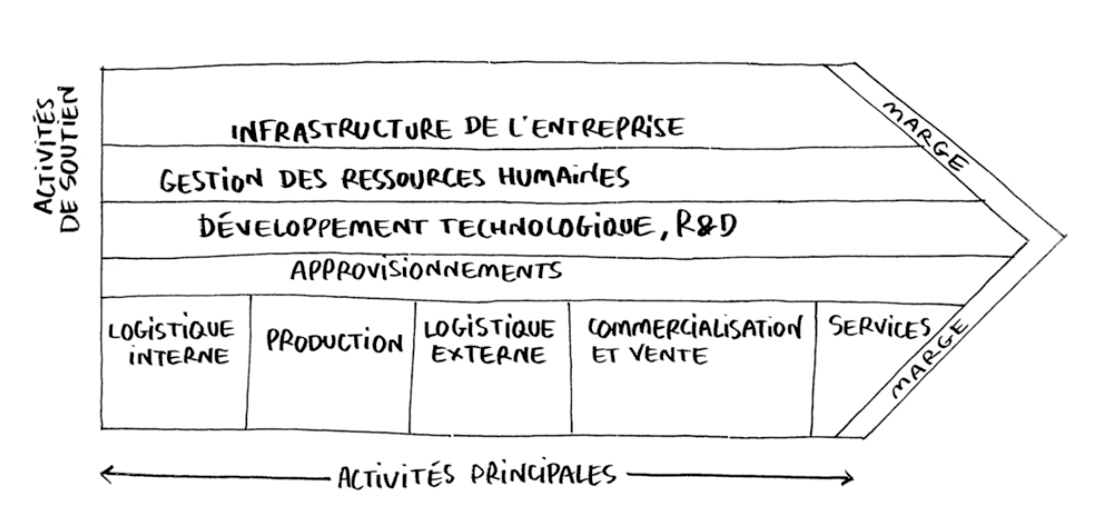
\includegraphics[scale = 0.70]{img/chaine_de_valeur.jpg}
    \caption{Chaîne de valeur}
    \label{chaine_de_valeur}
\end{figure}
\\
La chaîne de valeur permet :
\begin{enumerate}
    \item d'identifier les activités de votre entreprise ;
    \item de comparer la valeur créée par chaque activité ;
    \item de comparer la valeur créée à celles de vos concurrents;
    \item et d'aider à la décision des activités à garder et des activités à faire réaliser par les autres.
\end{enumerate}
Les éléments obtenus se traduiront soit par une logique de coût, soit par une logique de valeur.\\
\\
Ce modèle de la chaîne de valeur est une étape parmi d'autres au sein de la filière industrielle (ou système de valeurs). Cette dernière représente l'ensemble des relations entre les différentes entreprises nécessaires à la création, la production et la vente d'un produit/service.
\subsection{L'inimitabilité de l'avantage concurrentiel}
Nous pouvons voir les différentes stratégies qu'une entreprise peut mettre en place pour se protéger des imitateurs. On retrouve les moyens réglementaires (e.g. les systèmes juridiques), l'art de la discrétion ou limiter l'imitation (en prenant, e.g., une position monopolistique). Néanmoins, ces trois moyens traitent les symptômes et non les causes. Ces dernières peuvent être traité en créant une complexité de coordination (traduit par l'ambiguïté causale) ou une culture d'entreprise. Mais il convient de ne pas confondre imitabilité et réplicabilité. 
\section{Les stratégies business}
\subsection{Les stratégies génériques de Porter}
Une stratégie générique\footnote{Les stratégies génériques, stratégies concurrentielles et business stratégies font référence au même type de stratégie.} désigne le mode d'action mis en oeuvre par l'entreprise pour développer son avantage concurrentiel. Michael Porter décline les stratégies génériques en trois grandes catégories.\footnote{Chaque stratégie concurrentielle se définit au sein d'un même DAS. Un travail d'identification des DAS est donc nécessaire au préalable.}
\subsubsection{La stratégie de domination par les coûts}
L'entreprise assure une supériorité sur ses concurrents en termes de coût. Elle développe une structure de coût durablement inférieur à celle de ces concurrents à l'aide principalement des économies d'échelle. Néanmoins, il existe d'autres mécanismes pour diminuer les coûts comme les économies de champs (moins coûteux de gérer plusieurs produits conjointement) ou l'effet d'expérience.\\
L'indicateur clé de cette domination par les coûts est celui de la part de marché.
\begin{ex}[McDonald's]
L'entreprise McDonald's a réussi à percer grâce à une domination par les coûts en introduisant dans le domaine de la restauration la production en série.
\end{ex}
\subsubsection{La stratégie de différenciation des productions/services}
Cette stratégie se fonde sur la capacité de l'entreprise à développer des caractéristiques distinctives des produits/services proposés. L'entreprise s'appuie sur des modes de concurrence hors prix, c'est-à-dire sur la création d'un ensemble de caractéristiques autres que le prix du bien. 
\begin{ex}[Apple]
Les ordinateurs de la marque sont vu comme des objets de design en plus d'être des ordinateurs.
\end{ex}
La différenciation se base également sur la capacité de l'entreprise à créer des produits/services qui correspondent à des attentes diverses. 
\begin{ex}[Grande distribution]
Les produits de grande distribution illustre ce concept. Combien de shampoings différents pouvez-vous trouver dans le commerce selon la couleur de vos cheveux ou leur nature ?
\end{ex}
Enfin, la différenciation peut reposer sur la rareté des ressources et des compétences qui permet de définir une offre unique. Cette offre aboutit à un sur-prix. 
\begin{ex}[Lacoste]
Lacoste peut se permettre de vendre ses polos à prix très élevés parce qu'il apprécie la qualité de la marque.
\end{ex}
\subsubsection{La stratégie de focalisation ou de niche}
Cette troisième stratégie propose de construire l'avantage concurrentiel sur la capacité de l'entreprise à satisfaire à sa clientèle (spécifique) de manière durable.
\begin{ex}[Tetra]
L'entreprise Tetra est leader mondiale dans l'aquariophilie avec une part de marché trois fois supérieure à celle de son premier concurrent.
\end{ex}
Les stratégies génériques de Porter ont tout de même plusieurs limites : cette typologie sert essentiellement dans les secteurs de l'industrie manufacturière ; elle fonctionne mieux dans les secteurs de grande consommation ; et elle repose sur une approche monolithique de la chaîne de valeur.
\subsection{L'horloge de Bowman}
Faulkner et Bowman ont élargi la typologie de Porter en proposant huit stratégies.\footnote{Nous pouvons regrouper ces stratégies en cinq groupes : stratégies de différenciation, stratégie de prix bas, stratégie hybride, stratégies de niche et stratégies vouées à l'échec. Ces dernières, étant une catégorie de stratégies perdantes ne seront pas abordées dans ce cours.} Nous allons nous baser sur leurs travaux pour construire une espace concurrentiel autour de deux critère : le prix et la valeur perçue. Mais il faut d'abord définir une offre de référence. Celle-ci repose sur un jugement subjectif des consommateurs qui évaluent un rapport qualité-prix considéré comme "juste."
\subsubsection{Les trois stratégies de différenciation}
Nous distinguons d'abord la stratégie dite de différenciation avec prix supérieur (par le haut) ou "premium." L'entreprise se concentre sur la création de la valeur perçue.
\begin{ex}[BMW]
BMW bénéfice d'une valeur perçue supérieur à l'offre de référence grâce à ses voitures fiables, robuste et design. La société demande donc un prix supérieur.
\end{ex}
Deuxièmement, nous distinguons la stratégie de différenciation sans pris supérieur (par le haut) ou "sophistication." Cette stratégie propose une valeur perçue supérieur sans pour autant augmenter les prix.
\begin{ex}[Automobile]
Des années de garantie pièces et main-d'oeuvre gratuites proposées par un constructeur automobile à ses clients constituent une forme de stratégie de sophistication.
\end{ex}
Enfin, nous distinguons la stratégie de différenciation avec prix inférieur (par le bas) ou "épuration." Celle-ci cible les clients en proposant un prix moindre avec une valeur perçue moindre également. 
\begin{ex}[Logan]
La voiture Logan lancée par Renault est un bon exemple de stratégie d'épuration car elle est aujourd'hui proposée à un prix inférieur à 5.000 euros.
\end{ex}
\subsubsection{La stratégie de prix bas}
Cette stratégie propose de vendre un produit/service à moindre prix pour une valeur perçue par le client égal à l'offre de référence (e.g. Walmart). Cette stratégie nécessite de détenir de grande part de marché parce que doit disposer de capacités financières suffisantes pour réduire les marges ou de capacités de négociation importantes. 
\subsubsection{La stratégie hybride}
Cette stratégie consiste à réduire le prix d'un produit/service tout en assurant une valeur perçue par le client supérieure à l'offre de référence (e.g. Ikea avec sa formule en kit). Ce positionnement nécessite une capacité à générer un surplus de valeur tout en optimisant ses coûts de production, ses coûts de distribution et l'ensemble de sa chaîne de valeur.
\subsubsection{Les stratégies de niche}
On peut identifier deux stratégies de niche ou de focalisation: par le haut et par le bas. Ces stratégies constituent des formes de différenciations extrêmes\footnote{Lors de l'examen de Janvier 2018, il a été discuté si ces stratégies pouvaient entrer dans les stratégies de différenciation. Le professeur Alain Vas \it{"considère qu’elles ne doivent pas entrer dans la réponse mais [il] admet que l’on puisse défendre le point de vue d’intégrer la stratégie de focalisation par le haut comme cas de différenciation « extrême ».  En effet, les travaux fondateurs de Michael Porter présentent une stratégie de focalisation par la différenciation (vers le haut) à côté de la stratégie de focalisation par la maîtrise des coûts (vers le bas).  Néanmoins, [il] rappelle que la question précise « en s’inspirant de Bowman » et non des travaux de Michael Porter. Selon l’argumentation apportée par l’étudiante ou l’étudiant, la réponse pourra être acceptée."}} Cette stratégie est proposée à un segment de clientèle spécifique en proposant un produit/service spécifique.
\begin{ex}[Ferrari]
Le positionnement haute gamme de Ferrari par rapport à une voiture européenne de type Renault Talisman se destine à une clientèle restreinte sensible à une expérience unique.
\end{ex}
\subsection{La stratégie Océan Bleu}
Distinguons, d'abord, l'océan rouge qui désigne l'approche traditionnelle d'un environnement concurrentiel connu dans lequel les entreprises s'affrontent pour gagner des parts du marché.
À l'opposé, l'océan bleu vise à relancer une activité dans un marché jugé saturé et hyper concurrentiel afin de développer de nouvelles perspectives de croissance. Quelques conseils peuvent être utile pour explorer la piste d'une stratégie océan bleu.
\begin{enumerate}
    \item S'inspirer des idées d'autres industries;
    \item explorer les attentes de certains consommateurs;
    \item examiner le produit au-delà de ses fonctionnalités;
    \item ou construire les nouvelles tendances.
\end{enumerate}
L'entreprise doit donc étudier la concurrence, analyser les FCS et construire le canevas stratégique.\\
\\
\subsubsection{La matrice ERAC}
L'entreprise doit également réfléchir sur la façon de faire évoluer les FCS à l'aide de quatre actions repris sous le nom de la matrice ERAC :  Exclure, Renforcer, Atténuer et Créer. 
\begin{ex}[Nespresso]
Nespresso a choisir d'exclure la distribution de ses produits en grande surface et de créer sa propre chaîne de magasins (Exclure). L'entreprise a augmenté la qualité perçue du café et a beaucoup investit dans la publicité (Renforcer). Le conditionnement en petites capsules individualisées ainsi qu'une variété plus limitées de cafés correspondent à une atténuation. Enfin, Nespresso développe ses propres points de vente et propose ses propres machines (Créer). 
\end{ex}
En conclusion, l'entreprise doit se focaliser sur un seul objectif en créant une divergence au niveau des règles classiques à l'aide d'un slogan percutant.
\section{Les stratégie corporate}
La stratégie corporate s'élabore au niveau de la maison mère et s'articule autour de quatre enjeux majeurs.
\begin{enumerate}
    \item Définir la mission de l'entreprise;
    \item définir le périmètre d'activité;
    \item définir la capacité stratégique du groupe à créer de la valeur dans ses DAS;
    \item et allouer les ressources au sein du groupe.
\end{enumerate}
On distingue deux grands type de stratégie corporate: la spécialisation et la diversification.
\subsection{La spécialisation}
Cette stratégie consiste à centrer toutes ses ressources et ses compétences dans un seul DAS. L'entreprise essaie de devenir leader et de bénéficier une rente de situation.
\subsubsection{Les avantages}
Les avantages offerts par cette stratégie sont :
\begin{enumerate}
    \item La sécurité de l'image de spécialiste,
    \item la capacité à développer un avantage concurrentiel fort,
    \item la capacité à bénéficier d'une taille critique,
    \item et la possibilité d'influencer le secteur.
\end{enumerate}
\subsubsection{Les désavantages}
La spécialisation présente des limites. L'entreprise peut devenir vulnérable :
\begin{enumerate}
    \item dans un contexte de demande saturée; 
    \item lorsqu'il y a trop de produits de substitution;
    \item lorsque survient un risque de rigidité organisationnelle;
    \item lorsque l'entreprise fait preuve d'un manque de capacité à capter les nouvelles innovations.
\end{enumerate}
\subsection{La diversification}
Cette stratégie consiste à répartir ses ressources entre les différents DAS.
\subsubsection{Les avantages}
Les avantages sont:
\begin{enumerate}
    \item la capacité à mobiliser des synergies,
    \item la capacité à améliorer la rentabilité,
    \item et la volonté de limiter les risques.
\end{enumerate}
\subsubsection{Les désavantages}
Les limites sont :
\begin{enumerate}
    \item un besoin en investissement et financement élevé,
    \item un risque de dispersion des ressources et compétences,
    \item et une gestion plus complexe.
\end{enumerate}
Il existe deux type de diversification : liée ou non liée. Dans le premier cas, l'entreprise crée une synergie entre ses DAS. Dans le second cas, aussi appelé diversification conglomérale, l'entreprise développe des activités sans points communs. Nous nous intéresserons qu'à la diversification liée. Elle repose sur deux types de synergies : les synergies commerciales et les synergies technologiques. On peut la subdiviser en deux types de diversification : horizontale ou verticale.
\subsubsection{Diversification horizontale}
Dans le cas d'une diversification horizontale, l'entreprise décide d'entrer dans de nouveaux secteurs donc les activités présentent des points commun avec son domaine initiale.
\subsubsection{Diversification verticale}
La diversification verticale repose quant à elle sur deux piliers : l'acquisition de nouvelles compétences et le renforcement de l'entreprise dans son domaine d'origine. L'intégration verticale en amont (esp. aval) consiste à intégrer le métier de ses fournisseurs (esp. client). 
Les avantages de ce type de diversification sont nombreux :
\begin{enumerate}
    \item Sécurité des approvisionnements et débouchés pour votre entreprise;
    \item réduction potentielle des coûts;
    \item maîtrise de technologies supplémentaires;
    \item internationalisation des marges;
    \item partage des informations;
    \item accroissement potentiel d'un pouvoir de marché;
    \item contrôle de la distribution;
    \item source de réactivité pour l'entreprise;
    \item et création de barrière à l'entrée.
\end{enumerate}
Les limites sont également nombreuses et sources d'échec.
\begin{enumerate}
    \item Les investissements peuvent s'avérer coûteux;
    \item la nécessité de maîtriser parfaitement les nouveaux métiers;
    \item la perte d'opportunités sur le marché;
\end{enumerate}
Ces stratégies posent toujours le mode de croissance qu'il faut privilégier : interne ou externe.
\subsection{La matrice d'Ansoff}
Cette matrice (cf. Figure \ref{ansoff}) représente les stratégies corporate et a pour objectif de faciliter la prise de décision.
\begin{figure}[ht!]
    \centering
    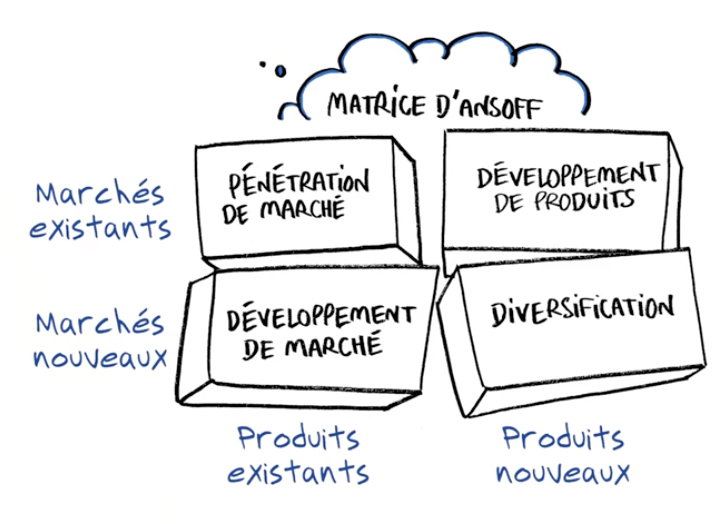
\includegraphics[scale = 0.8]{img/ansoff.jpg}
    \caption{Matrice d'Ansoff}
    \label{ansoff}
\end{figure}
\subsection{La matrice BCG}
Cette matrice (cf. Figure \ref{bcg}) a pour objectif de permettre aux dirigeants d'élaborer une stratégie corporate au niveau de leur groupe en intégrant l'idée d'un portefeuille d'entreprise équilibré. Elle constitue un outil d'aide à la décision.
\begin{figure}[ht!]
    \centering
    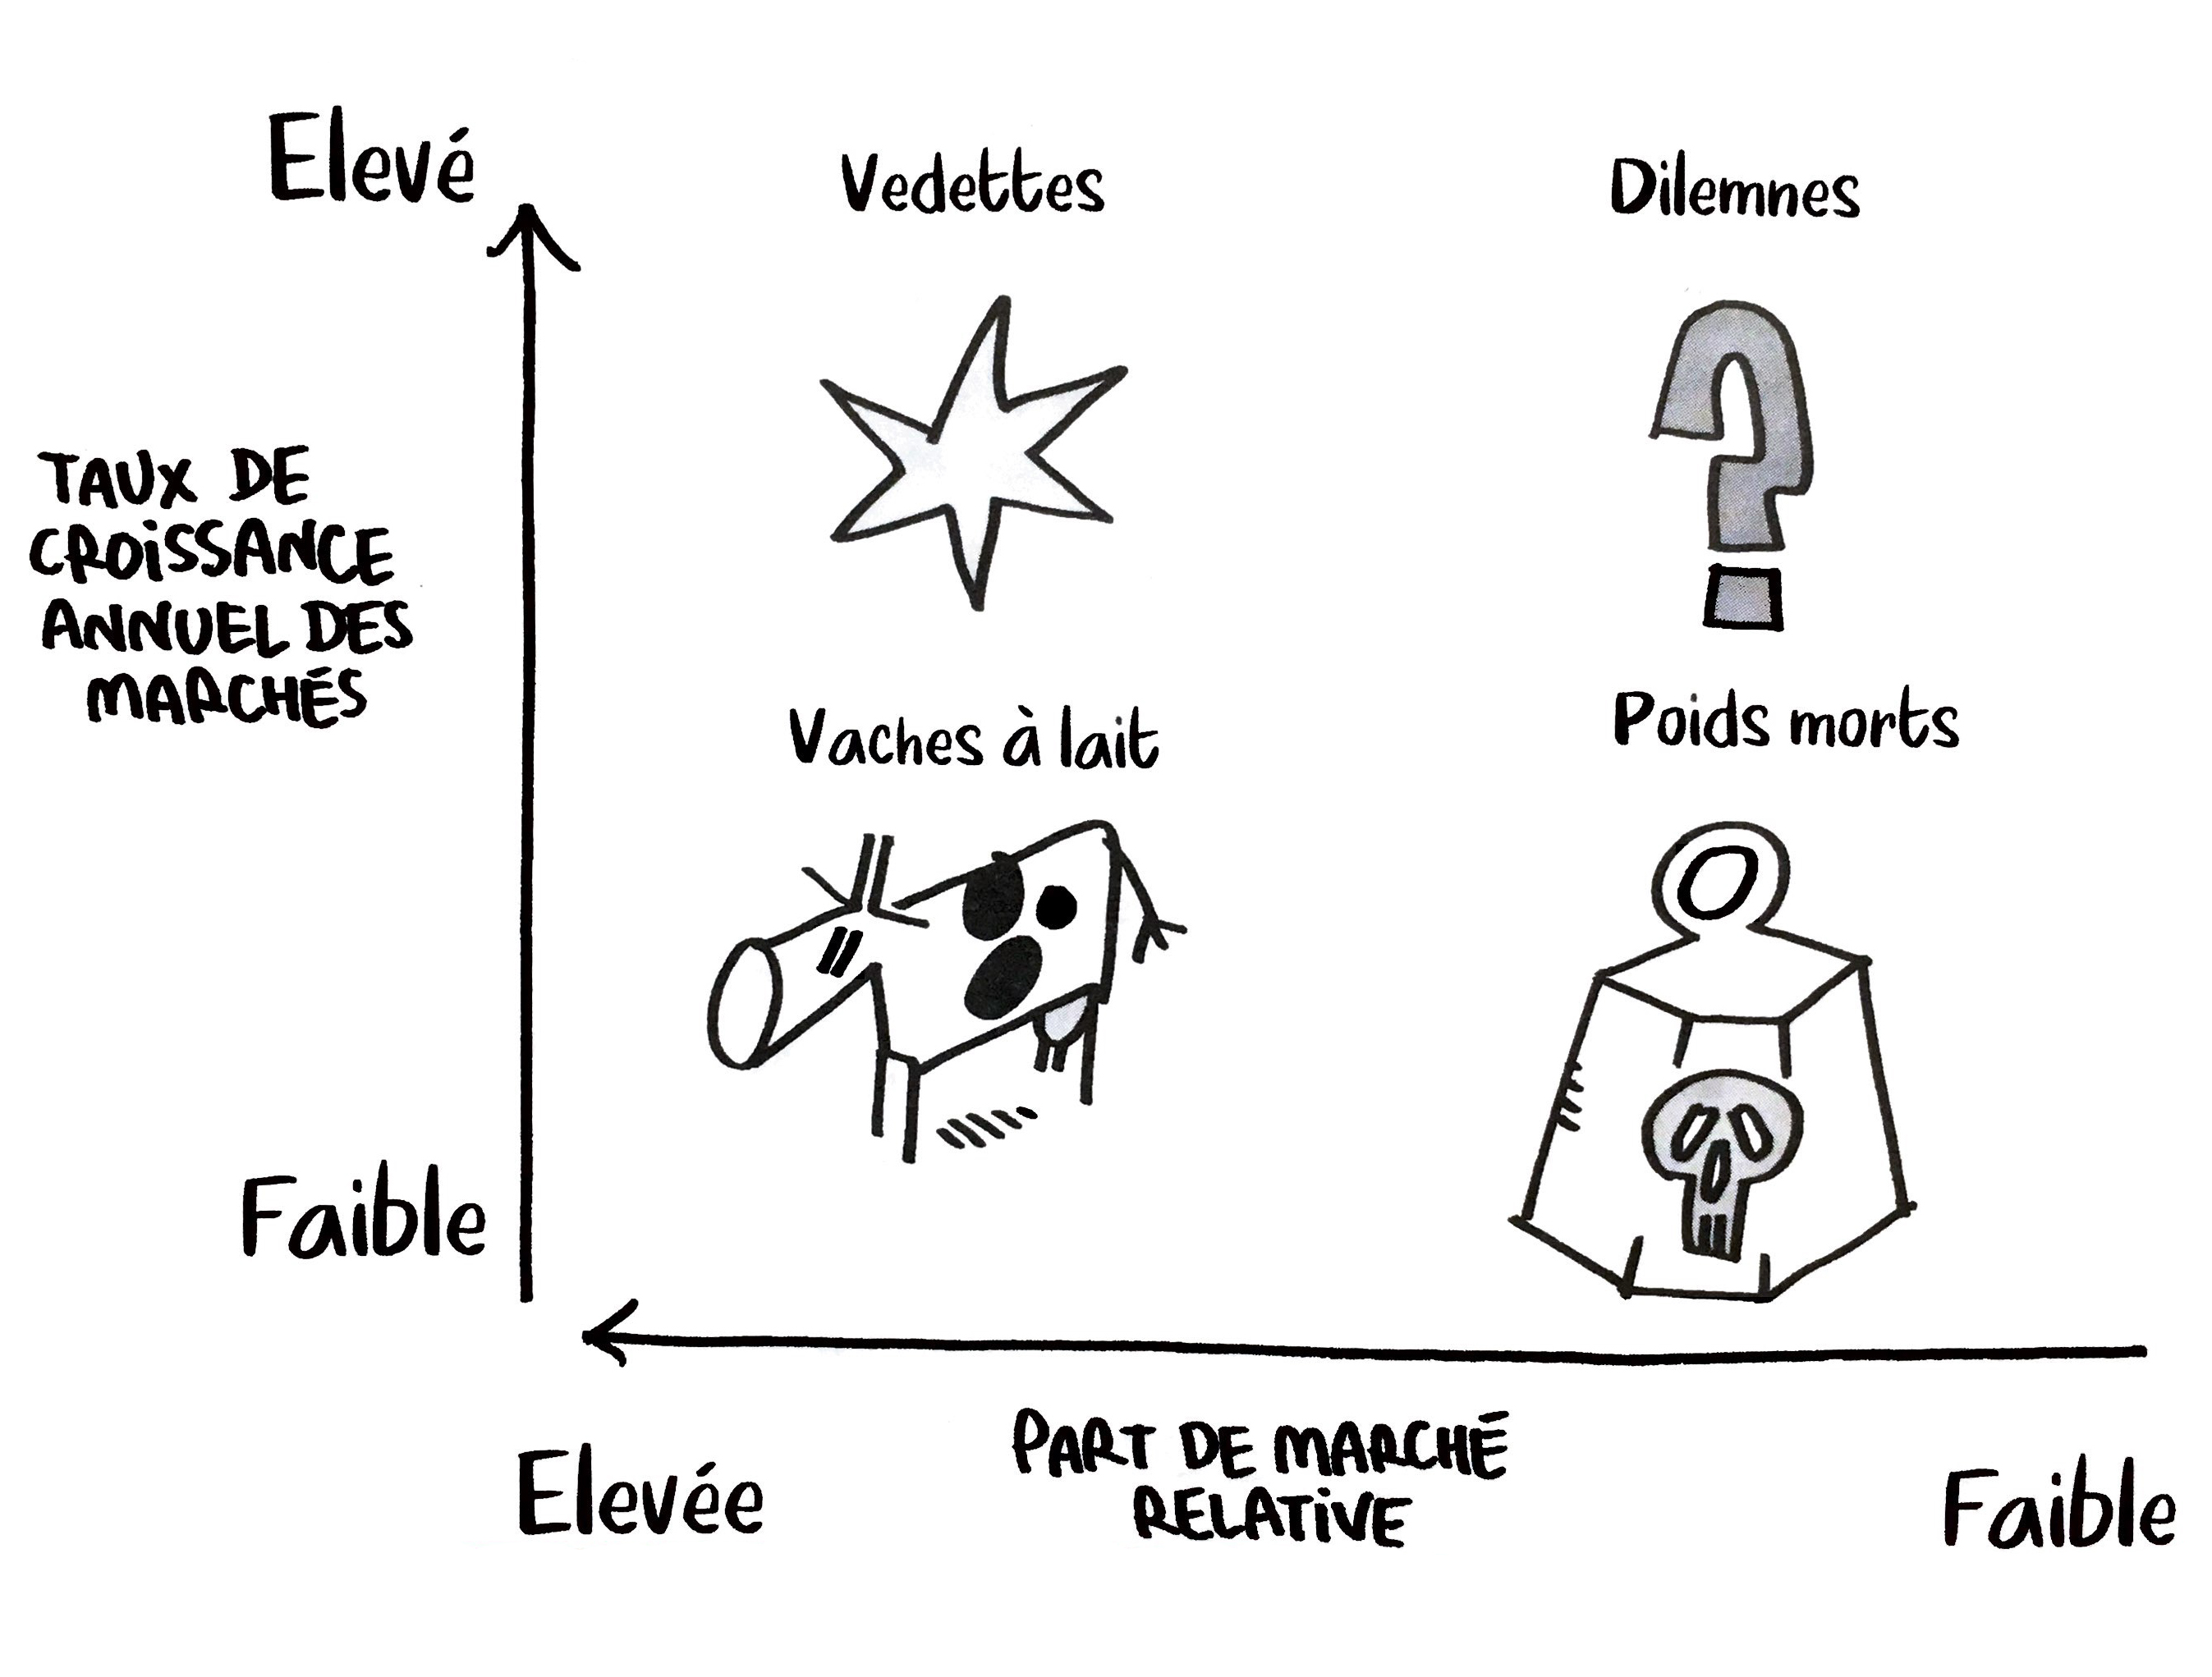
\includegraphics[scale = 0.4]{img/bcg.jpg}
    \caption{Matrice BCG}
    \label{bcg}
\end{figure}
On distingue quatre catégories dans la matrice BCG.
\subsubsection{La catégorie "vaches à lait"}
Dans cette catégorie, les besoins financiers sont limités et la position de leader sur le marché permet de faire des DAS une des sources importantes de liquidité.
\subsubsection{La catégorie "dilemmes"}
Dans cette catégorie, les DAS sont demandeurs de ressources financières et ils contribuent à la croissance de l'entreprise mais ils requièrent toujours des liquidités.
\subsubsection{La catégorie "Vedettes"}
Les DAS vedettes génèrent des ressources financières importantes et ils constituent la partie dynamique du portefeuille d'activités car ils sont en phase de croissance et sont destinés à devenir des vaches à lait.
\subsubsection{La catégorie "poids morts"}
Les DAS se caractérisent par un besoin faible de financement et par une création de liquidité tout aussi faible. Ils n'apportent pas de croissance et ne génèrent pas de marge. Il est conseillé de s'en débarrasser.
\subsubsection{Les besoins et limites de la matrice BCG}
Pour construire cette matrice, vous avez besoin des informations suivantes : 
\begin{enumerate}
    \item la taille et l'évolution du marché;
    \item votre part de marché;
    \item et le chiffre d'affaires annuel.
\end{enumerate}
Mais cette matrice à des limites telles que l'absence de prise en compte des interactions entre les DAS, la sous-estimation des interactions stratégiques. Elle repose sur une logique de volume et d'autofinancement.
\section{Les modes de développement}
Une entreprise qui développe avec succès une stratégie de groupe a l'opportunité de mettre en oeuvre une stratégie de croissance. Il en existe trois types : croissance interne, croissance par fusion ou acquisition et croissance par alliance stratégique.
\subsection{Croissance interne}
La croissance interne (ou croissance organique) désigne tout développement fondé sur les ressources et les compétences propres à l'organisation. 
Les raisons de privilégier la croissance interne sont les suivantes : 
\begin{enumerate}
    \item ressources et compétences uniques pour se protéger des risques d'appropriabilité;
    \item maintenir une grand homogénéité culturelle dans l'ensemble de l'organisation ;
    \item limiter les risques de surinvestissement en dosant la croissance interne selon les perspectives de croissance des opportunités de marché.
\end{enumerate}
Néanmoins, une croissance interne est par nature lente et coûteuse. Elle peut également entraîner l'entreprise sur un sentier de croissance difficile ajustable.
\begin{ex}[Nokia]
L'entreprise Nokia, leader mondiale de la téléphonie mobile dans les années 1990, s'est majoritairement développée en interne. Elle va rater le virage de l'internet mobile et plus généralement celui des smartphones.
\end{ex}
\subsection{Croissance par fusion et acquisition}
La fusion est le fait que deux ou plusieurs entreprises s'unissent pour créer une nouvelle entité. Au contraire, l'acquisition concerne l'intégration d'une entreprise dans le périmètre de l'entreprise acquéreuse.
Il existe plusieurs raisons de privilégier la fusion ou l'acquisition.
\begin{enumerate}
    \item Pour saisir des opportunités.
    \begin{ex}[Facebook]
    Facebook rachète Instragram pour intégrer avant les autres le partage de photographies dans son réseau social.
    \end{ex}
    \item Pour contourner des barrières à l'entrée.
    \begin{ex}[Banque]
    Dans le secteur bancaire, la pénétration de nouveaux marchés se fait le plus souvent par le rachat d'une banque déjà présente sur le territoire ciblé.
    \end{ex}
    \item Pour compléter les ressources et compétences.
    \begin{ex}[Pharmaceutique]
    L'industrie pharmaceutique a racheté les nouvelles entreprises et les laboratoires qui fleurissent dans le domaine de la biotechnologie.
    \end{ex}
    \item Pour apprendre.
    \item Pour une plus grande efficience des moyens de production.
    \item Pour une plus grande visibilité.
\end{enumerate}
Néanmoins, il existe deux grandes difficultés lors de ce type de croissance : le risque de surpayer l'entreprise ciblée et les difficultés organisationnelles et managériales.
\subsection{Croissance par alliance stratégique}
Lors d'une alliance stratégique, deux ou plusieurs entreprises réalisent un développement fondé sur les partage des ressources. Il en existe deux types : capitalistique et contractuelle.
Nous retrouvons trois grandes raisons de choisir ce type de croissance.
\begin{enumerate}
    \item Pour plus de diversité et d'efficience
    \item Pour plus de co-spécialisation
    \item Pour apprendre de nouvelles ressources et compétences.
\end{enumerate}
Il existe également trois grands types d'alliance stratégique. 
\subsubsection{Les alliances de pseudo-concentration}
Les entreprise développent, produisent et commercialisent un produit commun. Elles ont un objectif de taille et on observe généralement une seule chaîne de production.
\begin{ex}[Volkswagen \& Ford]
Les entreprises avaient créé une alliance de pseudo-concentration pour leurs premiers monospaces.
\end{ex}
\subsubsection{L'alliance complémentaire}
Les entreprises s'associent avec d'autres entreprises qui partagent des compétences et des attributions complémentaires. 
\begin{ex}[Renault Espace]
La Renault espace a été désignée par Matra qui se chargeait également de la carrosserie. Tandis que Renault s'occupait du moteur et du réseau de distribution.
\end{ex}
\subsubsection{L'alliance de co-intégration}
Elle associe deux entreprises visant à réaliser des économies d'échelle sur un composant ou à un stade du processus isolé.
\begin{ex}[Peugoet, Renault \& Volvo]
Les trois entreprises avaient opéré une alliance de co-intégration pour développer un nouveau moteur, le V6, dont ils pouvaient ensuite équiper leur véhicules.
\end{ex}
\section{Les cas étudiés}
Dans cette annexe, nous aborderons tous les cas étudiés au cours.
\subsection{Le cas Nintento}
Analysons les DAS de Nintendo (cf. Tableau \ref{DAS_nintendo}). Ils sont au nombre de deux : les consoles et les jeux.
\begin{table}[ht!]
    \centering
    \begin{tabular}{|x{5cm}|x{5cm}|x{5cm}|}
        \hline
        Critères externes & DAS consoles & DAS jeux\\
        \hline
        Clientèle & Grand public & Grand public \\
        \hline
        Critère d'achat & Fonctionnalité ludique et prix & Type de jeux et univers (e.g. Mario)\\
        \hline 
        Distribution & Grande surface, points de vente (spécialisés ou non) et internet &  Grande surface, points de vente (spécialisés ou non), internet et téléchargement\\
        \hline 
        Concurrence & Microsoft et Sony & EA, Ubisof, SquareEnix, etc.\\
        \hline
        Technologies & Micro-processeur, mémoire vive, carte graphique, système d'exploitation et manettes de jeu & Programmation informatique\\
        \hline
        Compétences & Informatique et électronique & Informatique, scénarios, design, etc.\\
        \hline
        Structure de coût & R\&D, matière première et assemblage & R\&D et développeurs\\
        \hline
    \end{tabular}
    \caption{Critères des DAS de Nindento}
    \label{DAS_nintendo}
\end{table}
Nous pouvons en tiré les facteurs clés de succès qui sont donnés dans le tableau \ref{FCS_nintendo}.
\begin{table}[ht!]
    \centering
    \begin{tabular}{|x{5cm}|x{5cm}|}
        \hline
        DAS consoles & DAS jeux\\
        \hline
        Prix inférieur à la concurrence pour les consoles portables  & Univers connu\\
        \hline
        Maîtrise des technologies & Portefeuille assez large\\
        \hline
        Expérience du joueur & Jeux qui s'adaptent à des profils de clients\\
        \hline
        Capacité d'innovation & Gameplay\\
        \hline
        Relations avec les éditeurs tiers & \\
        \hline
    \end{tabular}
    \caption{Facteurs clés de succès des DAS de Nintendo}
    \label{FCS_nintendo}
\end{table}
Nous pouvons maintenant identifier des synergies entre les différents DAS telles que
\begin{enumerate}
    \item Ventes couplées jeux-consoles (e.g. Zelda)
    \item Image et notoriété de la marque
    \item Même réseau de distribution
    \item Partage des compétence entre les DAS
\end{enumerate}
\subsection{Le cas Carrefour}
Analysons, dans un premier temps, le cas Carrefour en utilisant le modèle PESTEL.\\
\\
\bf{P}olitique : subventions et taxes, protection des consommateurs et soutien au commerce de proximité.\\
\bf{E}conomique : pouvoir d’achat, hard discount et montée en puissance des marques blanches.\\
\bf{S}ocio-culturel : changement des habitudes de consommation, évolution du commerce en ligne et changement du comportement des consommateurs.\\
\bf{T}echnologique : évolution du commerce en ligne.\\
\bf{E}nvironnement : consommation énergétique et provenance des aliments (e.g. label Bio).\\
\bf{L}égal : droit de la concurrence et  du commerce (loi Galland ayant pour but de protéger les petits fournisseurs et les petits commerces des réductions de prix que les grands fournisseurs offraient à leurs distributeurs ; loi Raffarin concernant la nécessité de demander une autorisation pour ouvrir un magasin de plus de $300\text{m}^2$).\\
On peut définir un modèle de filière industriel pour la grande distribution. Nous partirons des matières premières que nous diviserons en deux catégories : biens comestibles et biens non consommables.\\
\\
Analysons maintenant le modèle des cinq forces de Porter pour le cas Carrefour.
\begin{enumerate}
    \item Intensité concurrentielle : forte concentration.
    \item Concurrents directs : Leclerc, Auchan, hard discount (Aldi, Liddle).
    \item Menace des nouveaux entrants : Walmart mais il y a beaucoup de barrières à l'entrée.
    \item Fournisseurs : PME et multinationales.
    \item Clients : ménages.
\end{enumerate}
Nous pouvons analysé la sixième force de Porter qu'est l'état en expliquant qu'il est régulateur et internationaliste avec les lois Galland et Raffarin.\\
\\
On observe une faiblesse dans le modèle des forces de Porter parce que nous ne prenons pas en compte l’alliance avec Promodès qui fut décisive pour le groupe. Elle a fait gagner Carrefour en extension et en internationalisation.\\
\\
Les FCS de la grande distribution sont donc les suivantes.
\begin{enumerate}
    \item Au niveau de l’intensité concurrentielle : fidéliser le client en offrant un certain service, en développant des marques propres (e.g. Everyday).
    \item L'innovation (e.g. format des magasins).
    \item La maîtrise des négociations entre les centrales d’achat et les fournisseurs : si nous couplons cela à d’autres sources d’approvisionnement, alors l'entreprise est moins dépendante des fournisseurs et elle augmente ainsi sa possibilité de réalisation de profit.
\end{enumerate}
\subsection{Le cas d'Apple}
Construisons la chaîne de valeur de la marque Apple (cf. Figure \ref{chaine_de_valeur_apple}).
\begin{figure}[ht!]
    \centering
    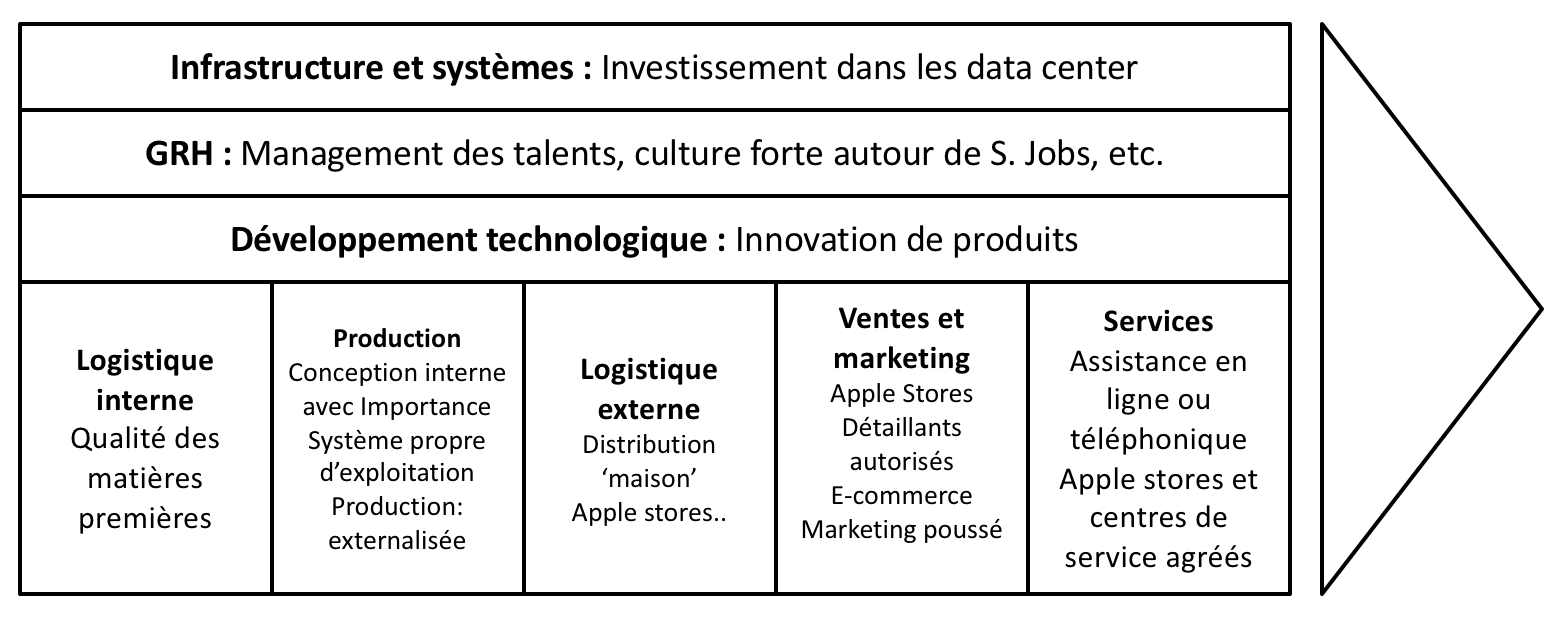
\includegraphics[scale = 0.6]{img/chaine_de_valeur_apple.png}
    \caption{Chaîne de valeur de Apple}
    \label{chaine_de_valeur_apple}
\end{figure}
Dans le cas d'Apple, les fonctions créatrices sont le développement technologique, la logistique interne et les ventes et marketing. 
\subsection{Le cas Dell}
Dans un premier temps, nous allons définir les ressources et compétences seuils ainsi que les ressources uniques et les compétences distinctives dans le tableau \ref{r_and_c_dell}.
\begin{table}[ht!]
    \centering
    \begin{tabular}{|x{4cm}|x{5cm}|x{5cm}|}
        \hline
        & Ressources & Compétences\\
        \hline
        Seuil & 
        \begin{enumerate}
            \item Personnel
            \item Bureaux, entrepôts, et usines
            \item Systèmes informatiques
            \item Centre d'appel
            \item Base de donnée clients
        \end{enumerate} & 
        \begin{enumerate}
            \item managériales
            \item informatiques
            \item commerciales
        \end{enumerate} \\
        \hline
        Uniques/Distinctives & 
       \begin{enumerate}
            \item Marque et notoriété
            \item Michael Dell
            \item Proximité des fournisseurs et des usines d'assemblage
            \item Gamme complète de produits/services
        \end{enumerate} & 
        \begin{enumerate}
            \item Vente direct
            \item Produits faits sur mesure
            \item Livraison à domicile
            \item Système Just-In-Time
            \item Prise de commande segmentée
            \item Gestion de données
        \end{enumerate}\\
        \hline
    \end{tabular}
    \caption{Ressources et compétences de Dell}
    \label{r_and_c_dell}
\end{table}
Nous pouvons maintenant donner la chaîne de valeur de la marque (cf. Figure \ref{chaine_de_valeur_dell}).
\begin{figure}[ht!]
    \centering
    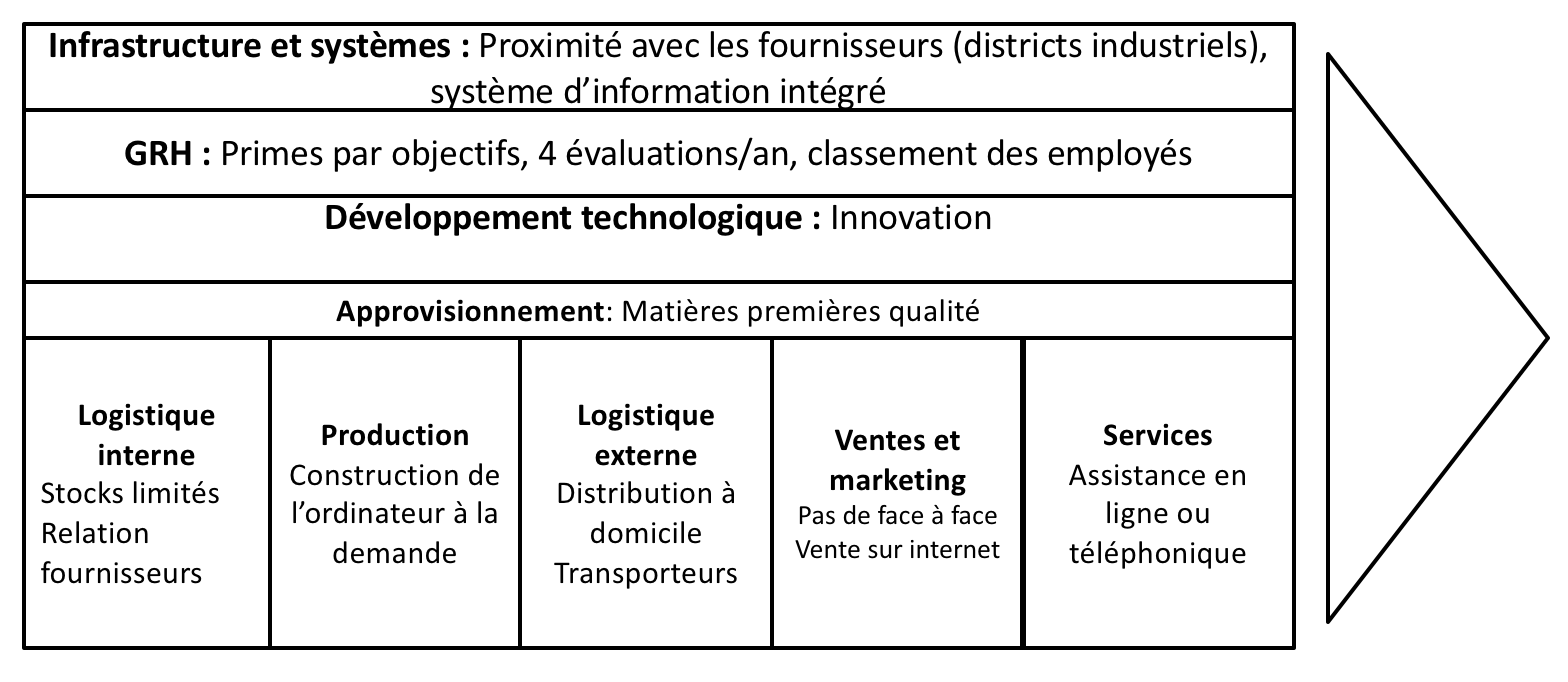
\includegraphics[scale = 0.6]{img/chaine_de_valeur_dell.png}
    \caption{Chaîne de valeur de Dell}
    \label{chaine_de_valeur_dell}
\end{figure}\\
\\
Les fonctions créatrices de valeur de Dell sont l'infrastructure et les systèmes, la production et les ventes et marketing. \\
Dell a réussi avec des concepts innovants tels que le Build to Order, la vente direct via internet et la personnalisation des ordinateurs.
\subsection{Le cas de Club Med}
Analysons, dans un premier temps, les DAS du groupe Club Med.
\begin{enumerate}
    \item Villages de vacances : offre all-in avec un certain confort et une certaine diversité, fidélisation des clients et grande présence sur internet.
    \item Circuits touristiques : proximité directe avec les locaux et tourisme responsable
    \item Business : activités ludiques de vacances mais possibilité pour un groupe de travail de se retrouver dans des lieux de rendez-vous spécifiques.
    \item Vacances patrimoines : biens de grande valeur situés à des emplacements stratégiques.
\end{enumerate}
L'entreprise a évolué depuis sa création. Il est intéressant de réaliser une rétrospective des différentes stratégies de l'organisation. \\
\\
Tout d'abord, le Club Med adoptait une stratégie de différenciation. L’espace stratégique était vierge, on était donc en océan bleu. Il sera considéré comme l’offre de référence.\\
\\
Par la suite, Marmara propose le même type de services. Le Club Med proposant un village pour vacanciers sous tente, sa valeur perçue en terme de confort était inférieure à celle du nouvel entrant. Le surprix que l’entreprise pratiquait n’était plus justifié.\\
\\
Club Med a ensuite subi une restructuration entre 1997-2002 avec le plan HGE. Il a opéré une stratégie de sophistication avec surprix en augmentant sa valeur perçue et son prix. Ce positionnement haut de gamme est en phase avec les évolutions de la concurrence et de la clientèle et l’implantation en Chine permet de cibler une nouvelle clientèle.
\section{Bibliographie} 
\bibliographystyle{plain}
\nocite{*}
\bibliography{references}
\end{document}
